\section{Análise do Cenário com Vento na Direção Y}

No cenário de vento na direção Y, analisamos as respostas dos ângulos de guinada, arfagem, e rolagem, bem como as coordenadas \(x\), \(y\) e \(z\). As análises detalhadas estão descritas a seguir.

\subsection{Guinada}

A Figura~\ref{fig:WindY-guinada} mostra a resposta do ângulo de guinada sob a influência de vento na direção Y. Observa-se que o valor de referência para a guinada permanece constante, enquanto os valores verdadeiro e estimado apresentam oscilações significativas em torno do zero. Essas oscilações indicam que o sistema está respondendo ao distúrbio do vento, e o controlador tenta estabilizar a guinada em torno do valor de referência, mas ainda apresenta uma pequena diferença entre o valor verdadeiro e o estimado.

\begin{figure}[H]
    \centering
    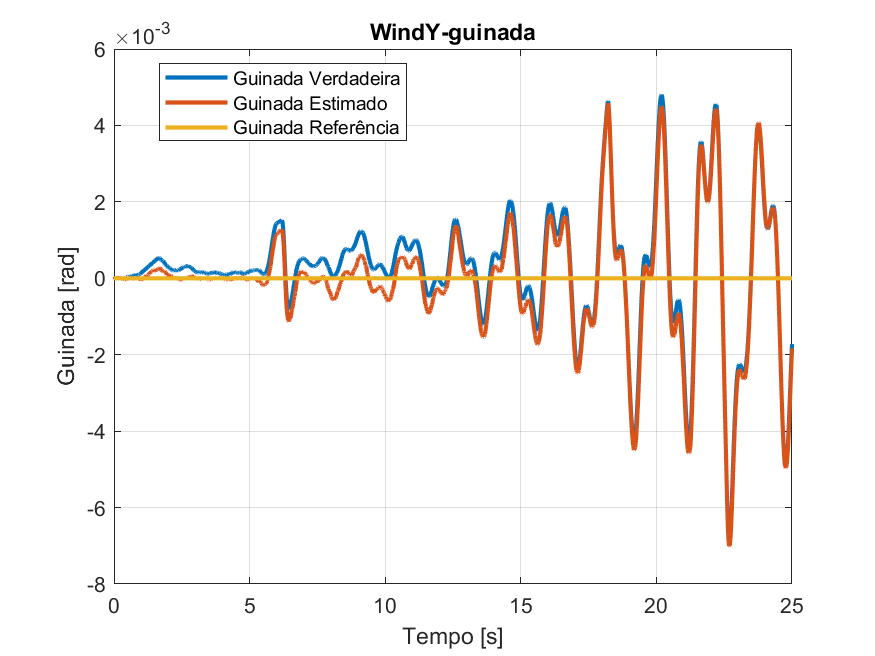
\includegraphics[width=0.6\textwidth]{WindY-guinada.png}
    \caption{Resposta da guinada para vento na direção Y}
    \label{fig:WindY-guinada}
\end{figure}

\subsection{Arfagem}

A Figura~\ref{fig:WindY-arfagem} ilustra o comportamento do ângulo de arfagem. O sistema apresenta uma resposta oscilatória com amortecimento na presença do vento. O ângulo de comando e o ângulo estimado seguem o valor de referência, com uma leve defasagem. Essas oscilações se estabilizam com o tempo, indicando que o sistema está buscando amortecer os efeitos do vento sobre o ângulo de arfagem.

\begin{figure}[H]
    \centering
    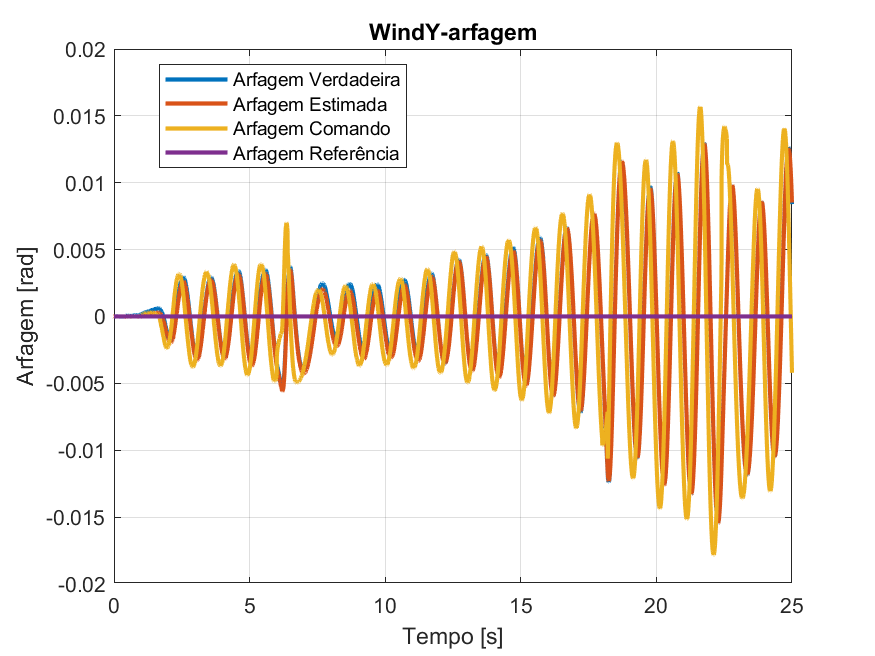
\includegraphics[width=0.6\textwidth]{WindY-arfagem.png}
    \caption{Resposta da arfagem para vento na direção Y}
    \label{fig:WindY-arfagem}
\end{figure}

\subsection{Rolagem}

A Figura~\ref{fig:WindY-rolagem} mostra a resposta do ângulo de rolagem. Nota-se uma oscilação amortecida, com uma resposta semelhante à observada na arfagem. O sistema busca compensar o efeito do vento ao longo do tempo, estabilizando o ângulo de rolagem próximo ao valor de referência.

\begin{figure}[H]
    \centering
    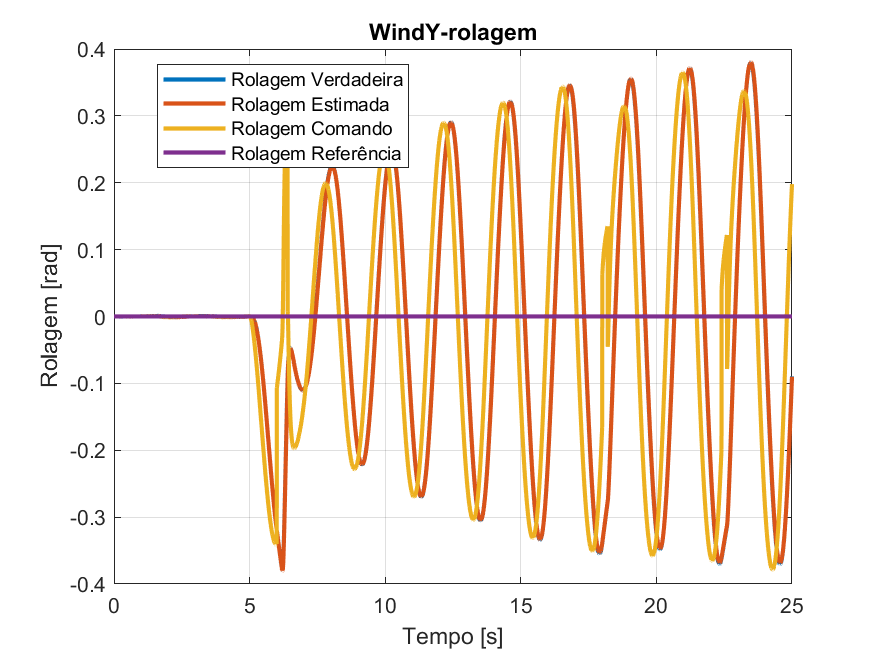
\includegraphics[width=0.6\textwidth]{WindY-rolagem.png}
    \caption{Resposta da rolagem para vento na direção Y}
    \label{fig:WindY-rolagem}
\end{figure}

\subsection{Coordenada Z}

Na Figura~\ref{fig:WindY-z} é apresentada a resposta da coordenada \(z\), indicando a altitude do sistema. Observa-se que o sistema mantém a altitude próxima ao valor de referência, com pequenas oscilações devidas ao distúrbio do vento. Esse comportamento demonstra que o controlador é eficaz na manutenção da altitude mesmo na presença de perturbações.

\begin{figure}[H]
    \centering
    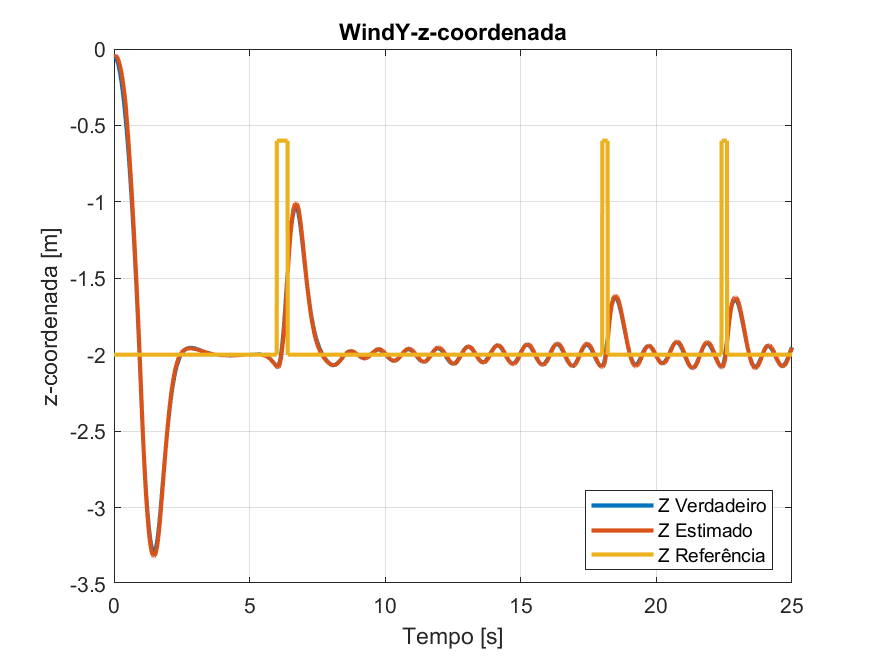
\includegraphics[width=0.6\textwidth]{WindY-z-coordenada.png}
    \caption{Resposta da coordenada Z para vento na direção Y}
    \label{fig:WindY-z}
\end{figure}

\subsection{Coordenada Y}

A resposta para a coordenada \(y\) é mostrada na Figura~\ref{fig:WindY-y}. Observa-se uma oscilação crescente ao longo do tempo, indicando uma resposta dinâmica à presença de vento na direção Y. O controlador tenta estabilizar a posição em Y, mas a influência do vento provoca uma oscilação significativa.

\begin{figure}[H]
    \centering
    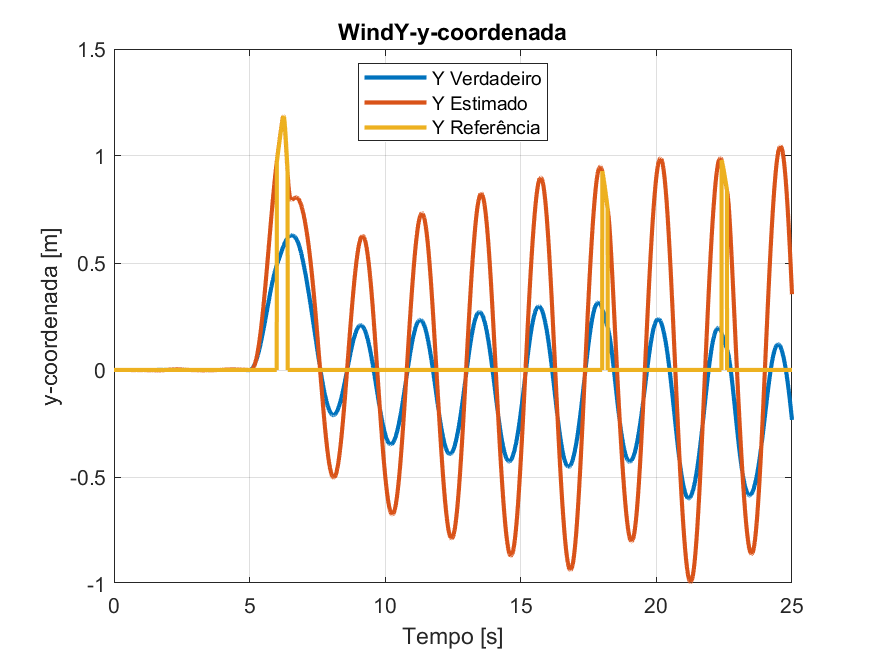
\includegraphics[width=0.6\textwidth]{WindY-y-coordenada.png}
    \caption{Resposta da coordenada Y para vento na direção Y}
    \label{fig:WindY-y}
\end{figure}

\subsection{Coordenada X}

Finalmente, a Figura~\ref{fig:WindY-x} apresenta a resposta para a coordenada \(x\). A resposta mostra uma pequena variação, indicando que o vento na direção Y tem uma influência limitada sobre a coordenada \(x\), com pequenas oscilações em torno do valor de referência.

\begin{figure}[H]
    \centering
    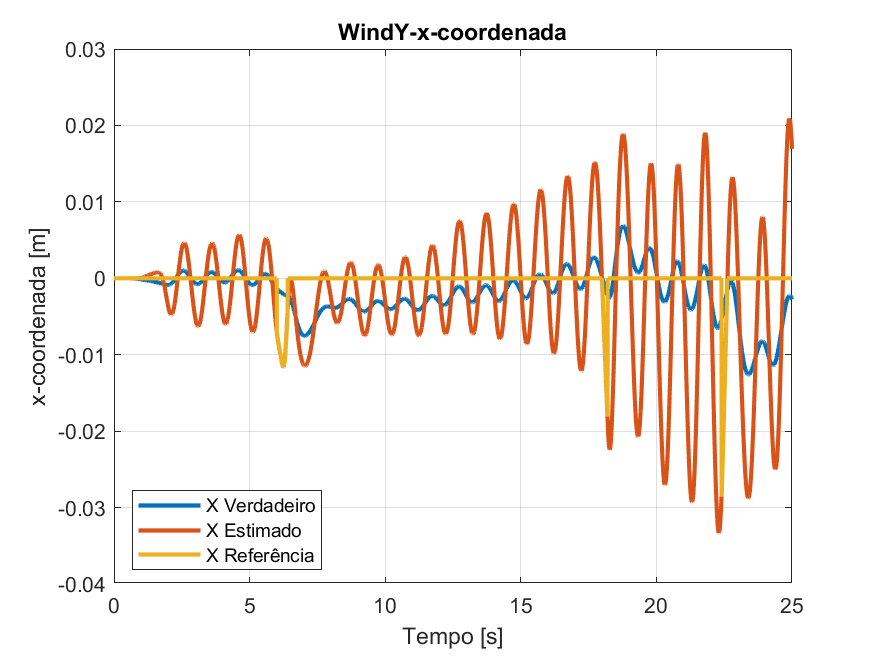
\includegraphics[width=0.6\textwidth]{WindY-x-coordenada.png}
    \caption{Resposta da coordenada X para vento na direção Y}
    \label{fig:WindY-x}
\end{figure}

%\subsection{Conclusão}

%A análise das respostas para o cenário de vento na direção Y mostra que o sistema apresenta oscilações significativas nos ângulos de guinada, arfagem e rolagem, bem como nas coordenadas \(x\) e \(y\). O controlador busca compensar o efeito do vento, especialmente nas coordenadas \(y\) e \(z\), mas ainda há oscilações residuais. A resposta do sistema evidencia a necessidade de um ajuste fino no controlador para minimizar os efeitos do vento nas diferentes direções.



%---------------------------------------------------------------------
% INDICE REMISSIVO
%---------------------------------------------------------------------
\phantompart
\printindex
%---------------------------------------------------------------------
